%!TEX root = ../main.tex
% -*- root: ../main.tex -*-
\section{Implementation}

Figure~\ref{fig:abstract-architecture} shows the proposed architecture for the computational continuum. Particular focus is put on the interaction between devices and Edge domain servers, since it is the main contribution of this paper. 
The main physical elements are mobile devices and domain servers. Mobile devices can be of any type (e.g., tablets, smartphones), running several low-latency applications that needs offloading part of their computation to more powerful servers. For this, the devices send information to be processed to the domain server through standardized network protocols~\cite{Sill17standards}.  A Base Transceiver Station\footnote{Different generations of wireless mobile networks use distinct names (e.g., eNodeB in 4G).} (BTS) bridges mobile devices and domain servers as a part of the cellular infrastructure and  Edge architecture, according to its current specifications~\cite{hu2015mobile}. In this scenario, mobile devices and Edge domain servers are at no more than a few hops from each other. These servers host a serverless infrastructure, where stateless functions are deployed and executed according to the phases defined by the A3-E model. 
The following sections provide details about the A3-E middleware (Section~\ref{subsec:A3-E}) and the serverless infrastructure that materializes Edge domain servers (Section~\ref{subsec:ServerlessArchCont}).


\begin{figure}[tbp]
	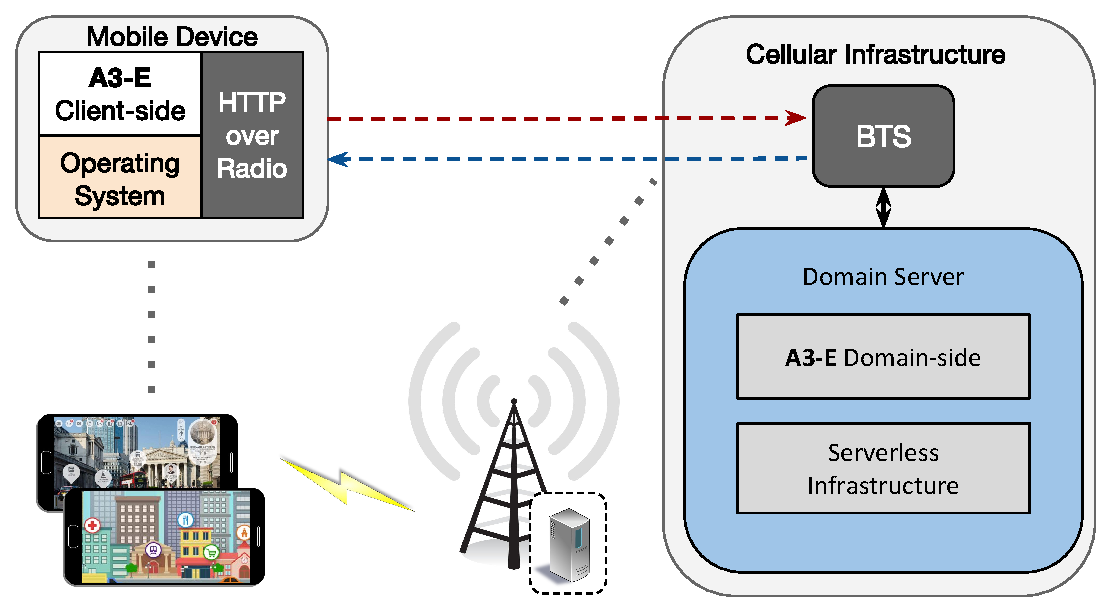
\includegraphics[width=.7\textwidth]{figs/Continuum_EdgeArch}
	\caption{A3-E architecture in Mobile Devices and Edge Domains}
	\label{fig:abstract-architecture}
\end{figure}

\subsection{A3-E Mobile Middleware}
\label{subsec:A3-E}

In order to assess the feasibility of the presented model and to validate it with an experimental evaluation we implemented a working prototype of the \textit{mobile middleware}. As described in Section~\ref{sec:proposal} this component interacts with  domains that could be either discoverable using a DNS-like mechanism or advertisement. The prototype is one of the possible materializations of the A3-E model, therefore it embraces the computing continuum: client applications can invoke functions without knowing where they will be actually executed (either locally, in one of the surrounding edge servers or in the cloud). The selection algorithm is based on the functions requirements, the domains availability and a multi-objective decision algorithm that will be described in the following. The implementation\footnote{Documentation and source code are available at \url{https://github.com/gioenn/a3e-android}} was written in Java for the Android operating system but could be easily generalized to any mobile platforms. 
\begin{figure}[tbp]
	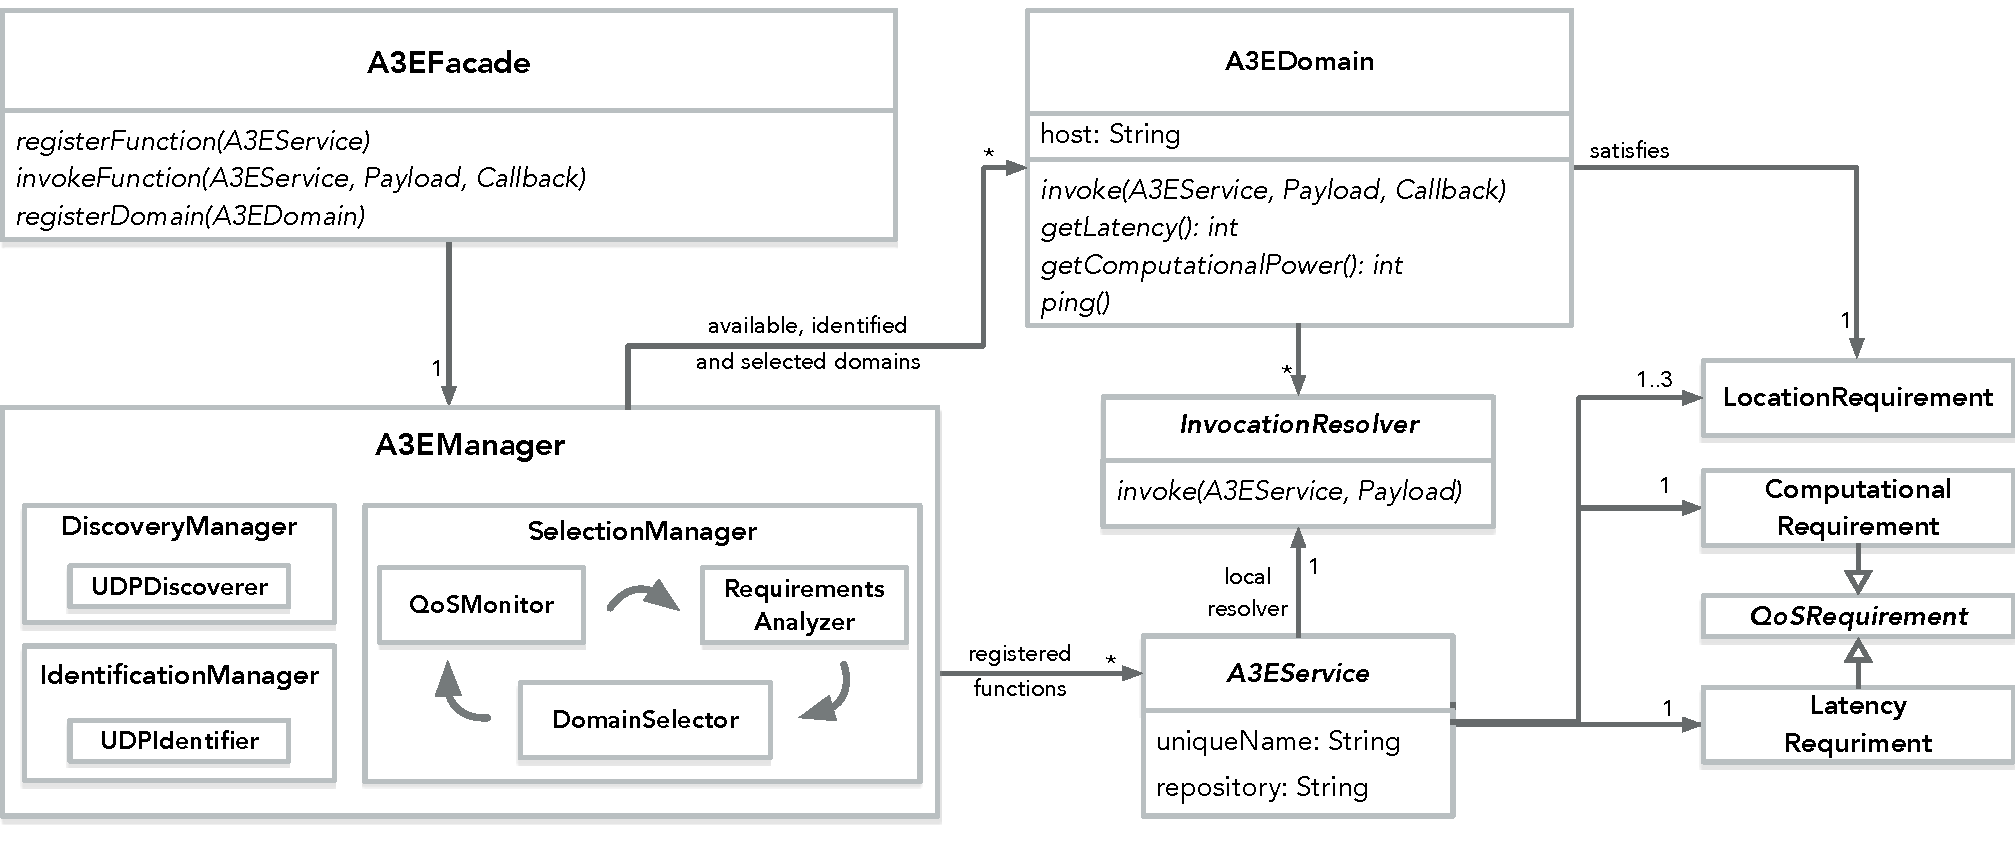
\includegraphics[width=1\textwidth]{figs/a3e-mobile-prototype}
	\caption{Mobile Middleware Architecture}
	\label{fig:mobile-prototype}
\end{figure}

Figure~\ref{fig:mobile-prototype} shows the architecture of the client middleware using an UML-like notation. Client mobile applications can support the continuum by simply interacting with two components:  \textit{A3EFunction}s and \textit{A3EFacade}. The former abstracts the actual functions to be executed, while the latter allows to first register and then execute functions. An \textit{A3EFunction} is identified by a unique name that corresponds to the name of the function asset that must be communicated to the continuum domains to be first acquired and then executed. Moreover each function must declare a set of non-functional QoS requirements that are organized in three types: 

\begin{itemize}
	\item \textit{Location Requirement}s are constrains over the continuum. A function can declare where it could be executed choosing a combination of three values: \textit{LOCAL}, \textit{EDGE} and \textit{CLOUD}. By default an \textit{A3EFunction} supports all three domain types but one can implement a function that, for example, cannot be executed locally thus only the \textit{EDGE} and \textit{CLOUD} requirements should be added.    
	\item \textit{Latency Requirement} expresses how important for a function is to have a low networking latency. The default value is \textit{LOW} since the main motivation of the work is to support low-latency applications. An \textit{A3EFunction}  can  also state that this requirement should be \textit{ANY} or \textit{VERY LOW}. The lower the latency requested the more the networking latency will be considered important in the the domain selection procedure.
	\item \textit{Computational Requirement} defines how relevant for a function is to have a fast computing processing. The predefined value is \textit{FAST}, since, again, the main targets of the approach are applications that requires fast request/response interactions. Similarly to the latency requirement two additional values are available:  \textit{ANY} or \textit{VERY FAST}. The higher  processing power is requested the more this metric will be considered important during the domain selection phase.
\end{itemize}

An \textit{A3EFunction} that support the \textit{LOCAL} location requirement should also define a local \textit{InvocationResolver}. As we are going to discuss later in this section, invocation resolvers deal with the invocation technology \textit{heterogenity}  of the continuum. For what regards the local domain we currently support the execution of native Java code and Javascript functions (that could be imported in the project as standard \textit{.js} files). For this purpose we created two \textit{InvocationResolver}s that can execute respectively Java or Javascript functions if the local domain is selected.  Finally before being able to execute it, the function must be registered using the \textit{A3EFacade}.

The \textit{A3EFacade} wraps the \textit{A3ELoopManager} that stores all the registered \textit{A3EFunctions} and manages a MAPE-inspired (Monitor, Analysis, Planning and Execution~\cite{kephart2003vision}) control loop for the discovery, identification and selection of domains corresponding to the \textit{Awareness}, \textit{Acquisition}, and \textit{Allocation} phases of the A3E model. The loop manager  consists of three main components called \textit{DiscoveryManager}, \textit{IdentificationManager} and \textit{SelectionManager}. 

The \textit{DiscoveryManager} explores the surrounding environment looking for available domains. An  \textit{A3EDomain} could be either \textit{static} or \textit{dynamic}. Static domains are added to the discovery manager at launch time, meaning that it is known a-priori that they will be available. Example of this are cloud and local domains. On contrary dynamic domains can be found only at runtime with appropriate technological protocols (such as DNS and advertising). Edge domains are not known a-priori thus they are considered dynamic. Static domains can be added by the client application using the \textit{registerDomain} operation provided by the \textit{A3EFacade} while dynamic domains are automatically discovered by the \textit{DiscoveryManager}.

 \textit{A3EDomain}s  are identified by an \textit{host} name, that is a unique network identifier by which it is possible to interact with the domain using a network. Moreover, as shown in the figure, a domain is considered \textit{Pingable} that means that it is possible to check for its availability and measure its networking latency (in milliseconds). Each domain satisfy a \textit{LocationRequirement}, intuitively local domains satisfies the \textit{LOCAL} requirement, while the edge and cloud ones the \textit{EDGE} and \textit{CLOUD} respectively.  A domain also provides three additional operations: one to execute a function within the domain, one to retrieve the networking latency (its value is lazily updated after a \textit{ping}) and one to obtain its computational power. Finally a domain also uses an \textit{InvocationResolver} to actually invoke the function. 
 
Therefore, in addition to find new domains, the \textit{DiscoveryManager} also checks for their availability pinging, at each control loop iteration, all the discovered domains retrieving their respective network latency. The output of this process is the list of the available domains. After that, the \textit{IdentificationManager} is activated. This component initializes the identification phase for each new available domain (e.g., domains discovered for the first time). For each new domain, the \textit{IdentificationManager} checks which registered functions can be executed on it (i.e., fulfillment of the location requirement), then it communicates with those functions (eventually triggering the allocation phase in the domain) and finally it retrieves its computational power. For this metric, in the current implementation, we are considering a fixed score ranging from $1$ to $5$ where the local domain is set to $1$, the edge domains to $4$ and the cloud ones to $5$. Labeling computational power is also common in the cloud where different tiers of virtual machines are available\footnote{\url{https://aws.amazon.com/ec2/instance-types/}} (e.g., micro, small, large). Note that in the continuum we label domains and not single machines and since the cloud has an infinite degree of scalability it gets the maximum score, independently of the machines in use. More sophisticated approaches, such as supporting dynamic scores that change according to the saturation of the domain or, in case of the local one, with respect to the battery level, are considered as future work.  

\begin{algorithm}[b]
	\caption{A3E Selection Algorithm}
	\label{alg:selection}
	\begin{algorithmic}[1]
		
		\Function{selectDomain}{A3EFunction $function$, A3EDomain[] $identifiedDomains$}
		\State$scoreRange \gets 5$
		\State $maxLatency \gets \Call{computeMaximumLatency}{identifiedDomains}$
		\State $maxCpuPower \gets \Call{computeMaximumComputationalPower}{identifiedDomains}$
		\State $latencyWeight \gets function.getLatencyRequirement()$ 
		\State $cpuPowerWeight \gets function.getComputationalPowerRequirement()$ 
		\State $maxScore \gets 0$
		\State $selectedDomain \gets null$
		\ForAll{$domain \in identifiedDomains$ } 
		\State $latency \gets domain.getLatency()$ 
		\State $cpuPower \gets function.getComputationalPower()$ 
		\State $latencyScore \gets latencyWeight*((scoreRange-1)*(1 - latency/maxLatency)+1)$ 
		\State $cpuPowerScore \gets cpuPowerWeight*(scoreRange*(cpuPower/maxCpuPower))$
		\State $score \gets (latencyScore + cpuPowerScore) / (latencyWeight + cpuPowerWeight)$
		\If{$score \geq maxScore$} 
		\State $maxScore \gets score$
		\State $selectedDomain \gets domain$
		\EndIf
		\EndFor 
		\State \Return $selectedDomain$
		\EndFunction
	\end{algorithmic}
\end{algorithm}

At the end of the identification phase, the networking latency and computational power of each domain is stored and the domain is considered ready to, eventually, execute functions (i.e., proactive approach). After that, the \textit{SelectionManager} starts the selection process for each function, as described in Algorithm~\ref{alg:selection}. The procedure is activated for each registered function with the identified domains (line $1$). The algorithm computes a score ranging from $0$ to $5$ (line $2$) for each domain and selects the highest one. The current implementation considers as quality metrics the networking latency and the computational power. The first step of the selection consists on computing the maximum latency and computational power (line $3$ and $4$) among the identified domains. This data, as already mentioned, were gathered during the previous phases. Then the weights of latency and computational power are retrieved (lines $5$ and $6$). These weights correspond to the values associated to the \textit{LatencyRequirement} and \textit{ComputationalPowerRequirement} of the function. The \textit{ANY} value corresponds to a weight of $0$, a latency requirement of \textit{LOW} and a computational power requirement of \textit{FAST} correspond to a weight equal to $1$, while weight equals to $2$ is considered for both latency \textit{VERY LOW} and computational power \textit{VERY FAST}.

For each domain, the algorithm computes the overall score (line  $9$ to $14$). The latency score is computed by normalizing the value retrieved at line $10$ with the maximum latency previously computed. The normalized value ranges from $0$ to $1$, the higher this value the higher the latency. Since a higher score should mean lower latencies, the algorithm computes the complement of this value and add $1$ to avoid scores equals to $0$. Finally, the latency score is computed to be in the range of $5$ and multiplied by the function's latency weight (line $12$). The computational power score is computed by normalizing the domain computational power retrieved at line $11$ with the  maximum value across the identified domains. Then the score for this metric is computed to be in the range of $5$ and multiplied by its weight (line $13$). Finally the overall score is computed by performing a weighted average between the scores obtained by the domains for the two QoS metrics.

Two considerations must be added for this algorithm. First, the procedure is an instantiation of the SMART approach~\cite{Olson1996} where multiple competing QoS objectives are considered in the decision process following the formula
\begin{equation}
Smart(c) = \frac{\sum_{i=1}^{n} QoSAtrribute_i(c)*weight_i)}{\sum_{i=1}^{n}weight_i} 
\end{equation}
where, the context of our approach, $c$ is a domain, $n$ is equal to $2$ and the QoS attributes values are networking latency and computational processing time.
Second, note that \textbf{the edge domains have the highest chances to be selected} (if available) since they usually combine a very low network latency and a medium to high computational power. 

After those steps, each function has its own selected domain that satisfies at best its requirements. At a control interval customizable by the user (default is $2$ seconds) the control loop restarts to look at possible new domains, the updated networking latency and, eventually, better selections.

The last phase to be described is the \textit{Engagement} phase where the actual function execution takes place. The client application can execute a function using the \textit{execute} operation of the  \textit{A3EFacade}. In addition to the \textit{A3EFunction}, the operation expects also a \textit{payload} (i.e., the function argument) that could be an object of any Java type, and a \textit{callback} since the execution is always asynchronous. The \textit{fa\c{c}ade} will then retrieve from the \textit{A3ELoopManager} the last selected \textit{A3EDomain} for the function. Since the control loop runs in a separated thread, the execution will not be affected if the selected domain changes during the invocation. After retrieving the best domain from the continuum, the \textit{A3EFacade} will execute the function by using the \textit{execute} operation of the \textit{A3EDomain}. Since each domains can use different technologies, the \textit{InvocationResolver} binded to the domain will be used to actually invoke the function. 

Invocation resolvers hide the technological details addressing the \textit{heterogeneity} property of the continuum. In the current implementation we created five types of \textit{InvocationResolver}s: two for executing local functions (either javascript or Java), one for Rest HTTP calls (this allows to support many FaaS platforms such as OpenWhisk\footnote{\url{https://github.com/apache/incubator-openwhisk/blob/master/docs/webactions.md}}), one specifically that exploit the AWS Lambda SDK\footnote{\url{https://aws.amazon.com/tools/\#sdk}} and finally a local invocation resolver that is binded to the local domain that simply forward the invocation to the function's local \textit{InvocationResolver} (either the \textit{JavaInvocationResolver} or \textit{JSInvocationResolver}). 

Since each function has its own characteristics, for example different REST calls could have different \textit{content-type}s and different format for input/output, we made each function able to modify the invocation with it is own applicative details. For this reason before invoking the actual function (e.g., performing the HTTP call) the \textit{InvocationResolver} creates a technology specific \textit{InvocationMean}. These components are wrappers to technology specific objects used by the invocation resolvers to build the call (e.g., the \textit{InvokeRequest\footnote{\url{http://docs.aws.amazon.com/AWSJavaSDK/latest/javadoc/com/amazonaws/services/lambda/model/InvokeRequest.html}}} object of the AWS Lambda SDK). As shown in Figure~\ref{fig:mobile-prototype} \textit{A3EFunction}s are \textit{InvocationMeanVisitor}s. Thus, just before performing the invocation, the specific \textit{visit} method is call providing to the function a way to fill up the request for the specific type of call. 

To summarize, supporting the continuum with A3E in a client application consists in the following four steps\footnote{A simple example of use can be found at \url{https://github.com/gioenn/a3e-android/blob/master/README.md}}:

\begin{enumerate}
	\item Register static \textit{A3EDomain}s such as cloud endpoints.
	\item Create \textit{A3EFunction}s and override the specific methods to customize the requests for the technologies of interest
	\item Register the functions
	\item Execute the functions in the continuum as plain programmatic calls 
\end{enumerate}

\subsection{Serverless Architecture for Edge Domains}
\label{subsec:ServerlessArchCont}

Following we briefly describe the serverless architecture that materializes the notion of Edge domains --- as shown in Figure~\ref{fig:domain-edge-arch}. 

\begin{figure}[htb]
	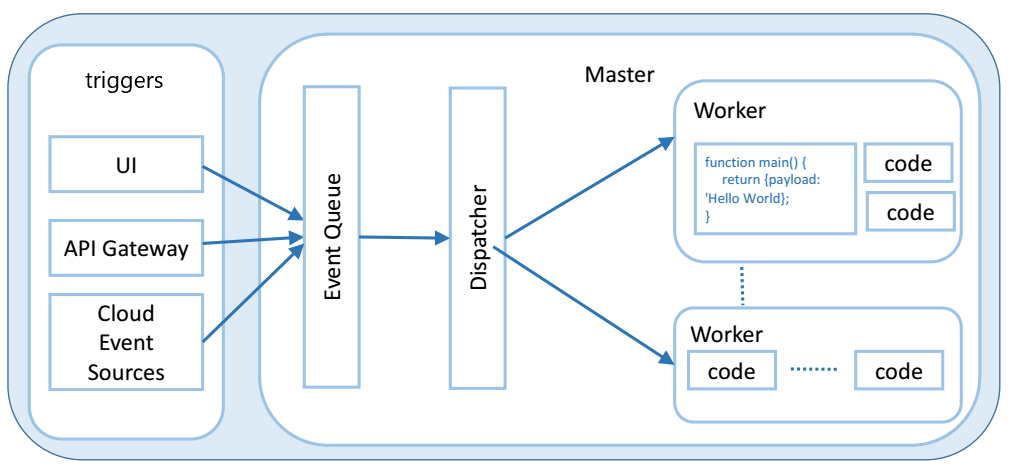
\includegraphics[width=.7\textwidth]{figs/ServerlessGenericArchEdit}
	\caption{Serverless Architecture in the Domain Server}
	\label{fig:domain-edge-arch}
\end{figure}

While Edge servers are ideal candidates for offloading the computation to preserve devices' battery life and reduce latency, these domain nodes are themselves potentially resource-constrained. Accordingly, the feasibility of hosting dedicated \textit{virtual machines}, \textit{containers}, and \textit{stateful applications} would also be limited, as these nodes cannot scale ``infinitely" to host always-running VMs/containers as the cloud itself. To overcome this limitation, we propose to materialize Edge domain servers through a serverless architecture~\cite{Roberts:2016,GarrigaMendonca2017}. 

Figure~\ref{fig:domain-edge-arch} details the serverless components deployed on the domain server. The entry points are the \textit{triggers} associated with events --- e.g.,  mobile sensor readings or HTTP requests from mobile apps.  
%in the MAR application, an event that triggers a function consists of uploading of an image or capturing a frame with the device's camera. --e.g., changes to database records, mobile sensor readings, code commits to a repository, or simple HTTP requests from Web or mobile apps. 
These triggers fire requests to an \textit{Http Server} that exposes available functions as REST endpoints. 

To achieve network transparency, a local Domain Name Server (DNS), deployed on the cellular infrastructure, must distinguish between requests addressed to the A3-E middleware/RESTful functions exposed by the domain server, and any other request for an Internet endpoint. The main difference from a regular DNS is locality, as the requests must be handled by the domain server on the current base station. To this end, the names of edge resources must be resolved locally without being propagated to public DNS servers. Whereas the specific details of the naming solution are outside the scope of this work, we argue that such a feature should not pose a significant technical challenge.% as it is already partially supported by the cellular infrastructure [CITE? is it right?].

Once a request reaches the domain server, it is then forwarded to a \textit{controller} component, which identifies and retrieves the function being called, authorizes the execution of such a function and identifies an available invoker to run it. \textit{Invokers} isolate the \textit{functions} in containerized environments, optimized and managed by the serverless provider to reduce overhead and response time. Note that cold starts can happen when the controller allocates an inactive/new function for the first time. It increases time for the first call while the provider provisions the invoker (runtime container) and then runs the function. However, when the function is still allocated or warm --- since it was engaged recently by the same or a different client --- the environment stays alive, ready and waiting for execution. Eventually, after a period of inactivity (that depends on the size of the function and the current load of the server), the provider can drop the container and the function be deallocated, freeing resources for other functions.


Finally, after execution, results and logging information are stored in the \textit{Storage} component, a highly available, noSQL database. Note that most of the components of the serverless architecture of the domain server are shared 
%(in grey in Figure~\ref{fig:abstract_architecture}) 
among all the functions. The highly shared nature and the automated management of the whole platform allows any function allocated on the domain servers to scale up automatically and elastically to unexpected bursts in the workload, and to scale down when it is not used anymore. In contrast with container-based stateful applications, the serverless platform is responsible for allocating functions of one or more applications on a pool of shared containers, according to the resources available at the domain server. As a result, the use of the computational resources of domain servers is optimized, allowing both more functions to be deployed and more requests to be processed simultaneously.

Needless to say, an IaaS/FaaS cloud domain can always be selected to allocate and engage functions when required --- due to unavailability/overload of edge domain servers. Their implementation is similar to those described above, although details can vary among different vendors\footnote{\url{https://github.com/apache/incubator-openwhisk/blob/master/docs/about.md}}.

As an advantage over the traditional, ``serverful'' approaches, it is not necessary to pre-allocate multiple virtual machines or containers to be resilient and responsive against downtime of single instances or bursts of workload. The on-demand execution of functions provides inherent scalability and optimal utilization as the number of running functions always matches the trigger rate. Additionally, the application developer only focuses on the application code and can fully outsource the management of the execution infrastructure to the A3-E middleware. The serverless approach also provides a fine-grained \textit{pay-per-use} billing model with benefits for both application owners and telecom operators (in charge of the domain servers).


